\documentclass[10pt,a4paper]{article}
\usepackage[utf8]{inputenc}
\usepackage[spanish]{babel}
\usepackage{amsmath}
\usepackage{amsfonts}
\usepackage{amssymb}
\usepackage{makeidx}
\usepackage{graphicx}
\usepackage{lmodern}
\usepackage{kpfonts}
\usepackage{fourier}
\usepackage[left=2cm,right=2cm,top=2cm,bottom=2cm]{geometry}
\usepackage[hidelinks]{hyperref}
\author{Luis Angel Torres Pinto.}
\title{Circuito de control de voltaje y corriente con tiristores.}
\begin{document}
\maketitle
\centering

\includegraphics[scale=2]{upzmg.jpg}\\
\raggedright
\newpage 
\section{Objetivo }
Esta practica consiste en controlar la intensidad de luz de un foco. Con el potenciómetro controlaremos gradualmente la intensidad de corriente que circula por el, haciendo que la intensidad del foco disminuya o aumente.
\section{Introducción.}
El triac es un dispositivo semiconductor de tres terminales que se usa para controlar el flujo de corriente promedio a una carga, con la particularidad de que conduce en ambos sentidos y puede ser bloqueado por inversión de la tensión o al disminuir la corriente por debajo del valor de mantenimiento. El triac puede ser disparado independientemente de la polarización de puerta, es decir, mediante una corriente de puerta positiva o negativa.\\
\bigskip 
Cuando el triac conduce, hay una trayectoria de flujo de corriente de muy baja resistencia de una terminal a la otra, dependiendo la dirección de flujo de la polaridad del voltaje externo aplicado.
Cuando el triac deja de conducir no puede fluir corriente entre las terminales principales sin importar la polaridad del voltaje externo aplicado por tanto actúa como un interruptor abierto.\\
\bigskip 
Debe tenerse en cuenta que si se aplica una variación de tensión importante al triac, aún sin conducción previa, el triac puede entrar en conducción directa.

\section{Materiales Utilizados. }
1.Foco\\
2.Triac\\
3.Diac\\
3.Potenciometro \\
4.Capacitor \\
5.Resistencia\\
6.Protoboard\\
7.Fuente de voltaje\\

\section{Procedimiento } 

Así quedara el circuito armado en protoboard.\\
\bigskip 
\centering
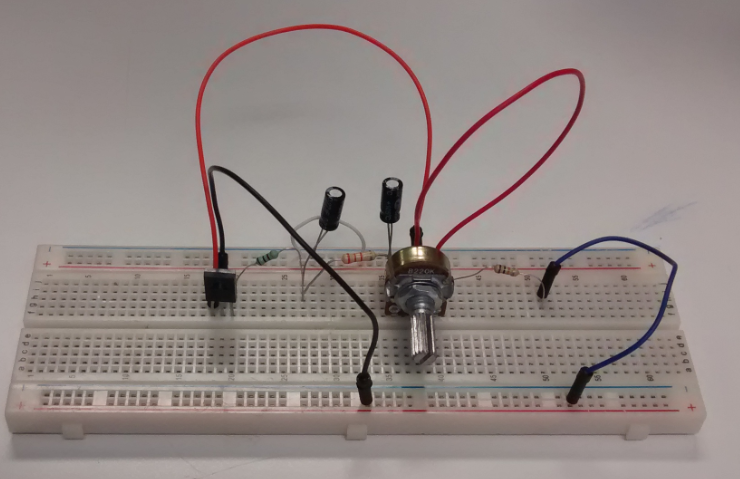
\includegraphics[scale=.80]{proto.png}\\
\raggedright
Así quedara el circuito armado en protoboard y conectado al foco, en este punto solo es de moverle al potenciómetro para que el foco disminuya la intensidad de luz.\\
\bigskip
\centering
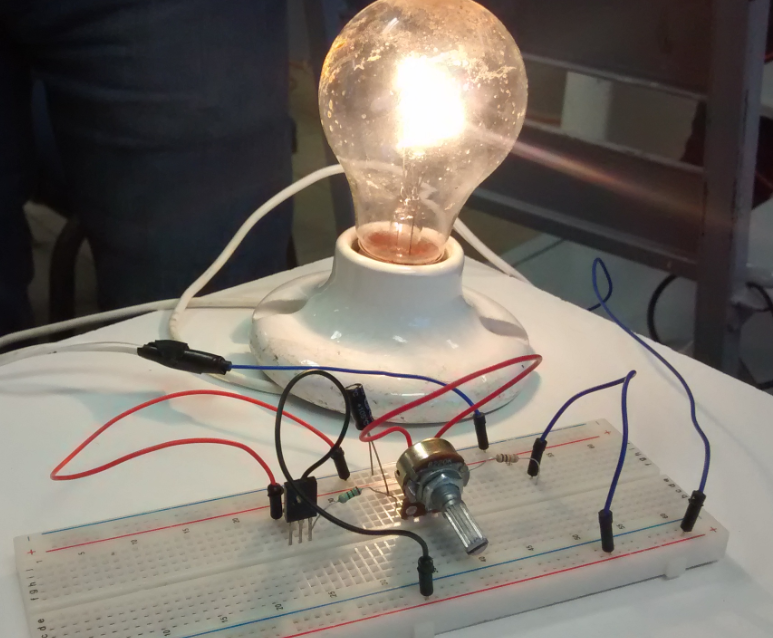
\includegraphics[scale=.70]{practica.png}\\
\raggedright

\section{Conclusión.}
Entre menor resistencia más intensidad, entre menor sea nuestra resistencia mayor es la intensidad y si disminuimos la resistencia la luz del foco se reflejara menos. Fue algo en lo que me di cuenta, ya que al principio nuestro circuito tenia una resistencia de 1k y la intensidad del foco era mayor, pero al aumentar más la intensidad de la luz con el potenciómetro quemaba la resistencia, por lo que se puso una resistencia mayor de 1.2k y en este caso la intensidad del foco al aumentar todo lo que nos permitía el potenciómetro, la luz no era tan intensa.\\
\bigskip
Cuando el TRIAC se bloquea se comporta como un interruptor cerrado.
\section{Bibliografía.}
Mecafenix, F. (22 de Octubre de 2018). Ingeniería Mecafenix. Obtenido de Ingeniería Mecafenix: \url{https://www.ingmecafenix.com/electronica/que-es-un-tiristor-y-como-funciona/}


\end{document}